% Minimal pandoc template for JCAP (jcappub.sty on article class).
% Engine: xelatex (STIX Two Text) so the prose Unicode + math render.
\documentclass[11pt,a4paper]{article}
\usepackage{iftex}
\ifPDFTeX
  \usepackage[T1]{fontenc}
  \usepackage[utf8]{inputenc}
\else
  \usepackage{fontspec}
  \setmainfont{STIX Two Text}
\fi

\usepackage{jcappub}   % loads amsmath, amssymb, graphicx, natbib[numbers], hyperref
\usepackage{orcidlink} % ORCID icon next to the author (hyperref already loaded by jcappub)

% --- prose Unicode operators -> math (works under xe/pdf latex) ---
\usepackage{newunicodechar}
\newunicodechar{→}{\ensuremath{\rightarrow}}
\newunicodechar{∂}{\ensuremath{\partial}}
\newunicodechar{∈}{\ensuremath{\in}}
\newunicodechar{∎}{\ensuremath{\blacksquare}}
\newunicodechar{□}{\ensuremath{\Box}}
\newunicodechar{∝}{\ensuremath{\propto}}
\newunicodechar{∞}{\ensuremath{\infty}}
\newunicodechar{∫}{\ensuremath{\int}}
\newunicodechar{≈}{\ensuremath{\approx}}
\newunicodechar{≠}{\ensuremath{\neq}}
\newunicodechar{≡}{\ensuremath{\equiv}}
\newunicodechar{≤}{\ensuremath{\leq}}
\newunicodechar{≥}{\ensuremath{\geq}}
\newunicodechar{≪}{\ensuremath{\ll}}
\newunicodechar{≫}{\ensuremath{\gg}}
\newunicodechar{≲}{\ensuremath{\lesssim}}
\newunicodechar{⊙}{\ensuremath{\odot}}
\newunicodechar{⅓}{\ensuremath{\tfrac{1}{3}}}
\newunicodechar{ₐ}{\ensuremath{{}_{a}}}
\newunicodechar{⊗}{\ensuremath{\otimes}}
\newunicodechar{⟹}{\ensuremath{\Longrightarrow}}
\newunicodechar{⟺}{\ensuremath{\Longleftrightarrow}}
\newunicodechar{⇒}{\ensuremath{\Rightarrow}}
\newunicodechar{⇔}{\ensuremath{\Leftrightarrow}}
\newunicodechar{𝓗}{\ensuremath{\mathcal{H}}}
\newunicodechar{√}{\ensuremath{\surd}}
\newunicodechar{∼}{\ensuremath{\sim}}
\newunicodechar{∇}{\ensuremath{\nabla}}
\newunicodechar{↔}{\ensuremath{\leftrightarrow}}
\newunicodechar{⟨}{\ensuremath{\langle}}
\newunicodechar{⟩}{\ensuremath{\rangle}}
\newunicodechar{−}{\ensuremath{-}}
\newunicodechar{ℓ}{\ensuremath{\ell}}
\newunicodechar{ħ}{\ensuremath{\hbar}}
\newunicodechar{′}{\ensuremath{{}^\prime}}
\newunicodechar{Ḣ}{\ensuremath{\dot H}}
\newunicodechar{Ṡ}{\ensuremath{\dot S}}
\newunicodechar{₊}{\ensuremath{{}_{+}}}

% --- pandoc body requirements ---
\usepackage{longtable,booktabs,array}
\usepackage{calc}
\usepackage{float}
\makeatletter
\newsavebox\pandoc@box
\newcommand*\pandocbounded[1]{%
  \sbox\pandoc@box{#1}%
  \Gscale@div\@tempa{\textheight}{\dimexpr\ht\pandoc@box+\dp\pandoc@box\relax}%
  \Gscale@div\@tempb{\linewidth}{\wd\pandoc@box}%
  \ifdim\@tempb\p@<\@tempa\p@\let\@tempa\@tempb\fi%
  \ifdim\@tempa\p@<\p@\scalebox{\@tempa}{\usebox\pandoc@box}%
  \else\usebox{\pandoc@box}%
  \fi%
}
\makeatother
\providecommand{\tightlist}{\setlength{\itemsep}{0pt}\setlength{\parskip}{0pt}}
\graphicspath{{../}{../figures/}{../../results/}}

% --- front matter (jcappub macros) ---
\title{Structural Entropy Dark Energy against DESI DR2, Pantheon+ and
Planck 2018: a zero-extra-parameter test}
\author{Stilian Pandev\,\orcidlink{0009-0005-8153-071X}}
\affiliation{Independent researcher}
\emailAdd{stilianpandev@gmail.com}
\abstract{We confront Structural Entropy Dark Energy (SEDE) --- a
structure-gated, H-linear horizon-entropy dark energy realized as a
cubic kinetic-gravity-braiding theory with braiding fraction b = 0.20
--- with the full DESI DR2 BAO, Pantheon+ SN, and Planck 2018 (lowl TT +
high-ℓ TTTEEE-lite) likelihoods, computed through the mochi-class
modified-gravity Boltzmann code inside cobaya. SEDE's background w(z) is
fixed by its reconstruction, so at the level of this comparison it
carries the \textbf{same free-parameter count as
\(\Lambda \mathrm{CDM}\)}. (This equal count is at the
background/geometry level; the perturbation sector adds one
\emph{disclosed} parameter, the braiding fraction b, registered as a
pre-committed falsifier measurable at ∼\(5\sigma\) by DESI DR3 + Euclid
--- not fit to the likelihoods driving this comparison.) At the
background level (BAO+SN+BBN) the two models are indistinguishable,
\(\Delta \chi ^{2} = -0.43\). With the full likelihoods, the best-fit
comparison gives
\(\Delta \chi ^{2}(\mathrm{SEDE}-\Lambda \mathrm{CDM}) = -3.4\), and
converged MCMC chains give a marginalized
\textbf{\(\Delta \mathrm{DIC} = -3.5\)} --- of which \(-3.0\) is the
mean-\(\chi ^{2}\) difference and the remaining half-unit an
effective-complexity term inside the Monte-Carlo scatter. At equal
parameter count SEDE is therefore \textbf{statistically consistent with
\(\Lambda \mathrm{CDM}\), with a mild same-direction pull}
\((\Delta \mathrm{DIC} \approx  -3.0\), ``positive but not strong''
evidence) residing entirely in the Planck high-ℓ likelihood, in the
direction of Planck's mild lensing-amplitude anomaly. Because that
anomaly is itself partly a lite-likelihood systematic, we test the pull
directly against the Planck 2018 lensing \((\phi \phi )\) likelihood in
a full BAO/SN/BBN-anchored joint refit \((\phi \phi\) as a best-fit
datum, separate from the DIC chains): it erodes the preference from
\(-3.5\) to \(-2.3\), consistent with about a third of the gain being
the \(A_{\mathrm{lens}}\) systematic rather than physical lensing --- we
make no detection claim. This is the SH0ES-free, full-likelihood
counterpart of the compressed-CMB preference reported in the companion
cosmology paper (there \(\Delta \mathrm{DIC} \approx  -3.5\) to
\(-4.7\), its upper end carried by the contested local-\(H_{0}\) prior
and the compression); the independent full-likelihood test here lands at
the conservative end, \(\Delta \mathrm{DIC} \approx  -3.0\). En route we
diagnose and fix a numerical pathology of the stable-parametrization
scalar sector (a spurious late-time oscillation seeded at the
GR\(\to\)EFT transition that mimics a large ISW signal), and we validate
the corrected pipeline exhaustively. SEDE's discriminating predictions
survive intact and are led by the one that does not depend on the solver
regime: a \textbf{+2--3\% scale-independent \(f\sigma 8\) enhancement}
through the RSD range --- fixed by the sub-horizon coupling
\(\mu _\infty  = 1.05\), independent of the tachyonic-window
regularization, opposite in sign to what would ease the \(S_{8}\)
tension, and within DESI DR3/Euclid reach --- with a corroborating
\textbf{−7.6\% ISW suppression} at ℓ = 2 (computed below the window and
correspondingly more model-dependent). The pipeline is rerunnable from
the released configurations and a pinned fork of the Boltzmann code (the
chain products and DIC-reduction script are to be committed with the
release; see Reproducibility).}
\keywords{dark energy theory; cosmological parameters from CMBR; baryon
acoustic oscillations; modified gravity}

% absorb small unbreakable-line overruns instead of margin overflow
\setlength{\emergencystretch}{3em}

\begin{document}
\maketitle
\section{Introduction}\label{sec-1}

SEDE posits that dark energy is the thermodynamic response of the cosmic
horizon with a volume-law (``Barrow \(\Delta  = 1\)'') entropy,
activated by the formation of cosmic structure through a saturation gate
\(f_{\mathrm{sat}}(\sigma _{\mathrm{R}}^{2})\). Its background history
is not a fitted \(w_{0}\)--\(w_{\mathrm{a}}\) curve: given the gate and
the entropy law, w(z) is produced by a fixed-point reconstruction (FPAB)
whose output --- a cubic KGB theory in the stable parametrization
\((\Delta M\)*², \(D_{\mathrm{kin}}\), \(c_{\mathrm{s}}^{2}\)), with
braiding \(\alpha _{\mathrm{B}} = b\cdot \Omega _{\mathrm{X}}\) and b =
0.20 (the adopted value; the QCD-derived braiding fraction is
\(b \approx  0.206\)) --- is then frozen. The model therefore enters a
likelihood comparison with \textbf{zero extra continuous background
parameters} relative to \(\Lambda \mathrm{CDM}\); its dark-energy sector
is either right or wrong as a shape.

The companion cosmology paper \citep{Pandev:2026cosmology} reports the
same mild preference from compressed CMB distance priors combined with a
local-\(H_{0}\) prior \((\Delta \mathrm{DIC} \approx  -3.5\) to
\(-4.7\), the upper end carried by the contested SH0ES prior and the
compression). Compressed priors plus a local-\(H_{0}\) prior are a
weaker foundation than the real likelihoods; the purpose of this paper
is to make the test as strong as we can --- the same question, asked of
the real likelihoods through the real Boltzmann hierarchy, with the full
posterior rather than a best-fit point, and SH0ES-free. It returns a
result \textbf{statistically consistent with \(\Lambda \mathrm{CDM}\)}:
a marginalized \(\Delta \mathrm{DIC} = -3.5\)
\((\Delta\)\(\langle\chi^2\rangle\) ≈ −3.0), a mild same-direction pull
at the conservative end of the companion's range.

Three results follow. First, the geometry:
\(\mathrm{SEDE} \approx  \Lambda \mathrm{CDM}\) on BAO+SN, as expected
for a background that tracks \(\Lambda \mathrm{CDM}\) to
\textbar1+w\textbar{} ≲ 0.01 at low z. Second, the full comparison: SEDE
is \textbf{statistically indistinguishable from
\(\Lambda \mathrm{CDM}\)}, with a mild same-direction pull
\((\Delta \mathrm{DIC} = -3.5\), \(\Delta\)\(\langle\chi^2\rangle\) ≈
−3.0) concentrated in Planck's high-ℓ TTTEEE, where SEDE's enhanced
growth supplies extra lensing smoothing in the direction of the
well-known \(A_{\mathrm{lens}}\) tendency
\citep{Planck:2018vyg, Calabrese:2008rt} --- a direction in which that
anomaly is itself partly a lite-likelihood systematic, so the origin of
the pull is left for the Planck lensing likelihood to decide, not
claimed here. Third, the predictions that make the model falsifiable
rather than merely fitting, led by the window-independent one: a +2--3\%
\(f\sigma 8\) signal fixed by the sub-horizon coupling at exactly the
scales DESI DR3 and Euclid measure, corroborated by \(a -7.6\)\% ISW
deficit at the lowest multipoles.

We also report, deliberately and in detail, a numerical failure mode of
the public modified-gravity solver in this regime and its resolution
(Section~\ref{sec-3}, Fig. 1): the previously adopted value of the
GR-transition redshift produced a grossly corrupted CMB spectrum which
briefly led us to retract the ISW prediction; the retraction was wrong,
the pathology is understood, and the guarded pipeline cannot silently
reproduce it.

\section{Model, pipeline and data}\label{sec-2}

\textbf{Model.} FPAB-SEDE \citep{Pandev:2026cosmology, Pandev:2026count}
at the b = 0.20 fixed point, a cubic kinetic-gravity-braiding theory
\citep{Deffayet:2010qz}. The background is supplied to the Boltzmann
code as tabulated \(\rho _\mathrm{DE}(a)\)
(\texttt{expansion\_model\ =\ rho\_de}) and the perturbation sector as
the stable-parametrization \citep{Bellini:2014fua} Chebyshev
coefficients (\texttt{gravity\_model\ =\ stable\_params},
\(\alpha _{\mathrm{B0}} = 0.139982\); the braiding
\(\alpha _{\mathrm{B}} = b\cdot \Omega _{\mathrm{X}}\) is the standard
density-tracking ansatz, with b = 0.20 in place of the generic 1.5).
Both files are frozen inputs, committed with the code fork. The gate in
\(\rho _\mathrm{DE}(a)\) is built from the \emph{background}
\((\mu  = 1)\) growth amplitude D(z) --- a functional of the expansion
history, not the solver's fifth-force-enhanced growth --- so the
tabulated background carries no hidden loop with \(\mu (k)\) (the H ↔
\(f_{\mathrm{sat}}(D)\) fixed point is closed separately to
\(10^{-13}\); cosmology paper §\ref{sec-2}). The effective gravitational
coupling at sub-horizon scales is \(\mu _\infty  = 1.051\) (1.05 to the
precision quoted in prose below); the gravitational slip is unity
\((c_{\mathrm{T}} = 1)\). To forestall a common misreading: SEDE is
\emph{holographic} dark energy --- \(\rho _\mathrm{DE}(a)\) enters an
otherwise standard-GR Friedmann background as a single added fluid ---
and mochi-class (a modified-gravity Boltzmann code) is used here only as
the perturbation solver for the cubic-KGB completion; SEDE itself is not
a modified-gravity theory of the background.

\textbf{Code.} mochi-class \citep{Cataneo:2024uox} (a
\(hi_{\mathrm{class}}\) \citep{Zumalacarregui:2016pph} descendant of
CLASS \citep{Blas:2011rf}) provides the modified-gravity Boltzmann
hierarchy; we drive it through cobaya 3.6.2 \citep{Torrado:2020dgo}. Two
pipeline details matter for anyone reproducing this: (i) cobaya must be
pointed at the modified-gravity classy build (\texttt{path:\ global}),
otherwise it silently loads a vanilla CLASS from its package path and
every SEDE evaluation fails; (ii) the perturbation sector requires the
GR-transition setting of Section~\ref{sec-3}. Our fork, including the
fix of Section~\ref{sec-3} and the frozen model inputs, is pinned at
commits \texttt{74d4b05} (solver guard) and \texttt{b365166} (inputs).

\textbf{Data.} DESI DR2 BAO \citep{DESI:2025zgx}
(\texttt{bao.desi\_dr2.desi\_bao\_all}); Pantheon+ SN
\citep{Brout:2022vxf} (\texttt{sn.pantheonplus}); Planck 2018 lowl TT
and high-ℓ \texttt{plik\_lite} TTTEEE \citep{Planck:2019nip} (clipy
implementation, validated against its test point to
\(4\times 10^{-9}\)). Gaussian priors: \(\tau  = 0.0544\) ± 0.0073; BBN
\(\omega _{\mathrm{b}} = 0.02218\) ± 0.00055 \citep{Schoneberg:2019wmt}
(applied identically to both models). Sampled parameters: \{\(H_{0}\),
\(\omega _{\mathrm{b}}\), \(\omega _{\mathrm{cdm}}\), log
\(A_{\mathrm{s}}\), \(n_{\mathrm{s}}\), \(\tau\)\} (six, identical for
both models); the \(plik_{\mathrm{lite}}\) calibration nuisance
\(A_{\mathrm{planck}}\) is held fixed at 1.0025.

\textbf{Spectral guard.} Every likelihood evaluation passes through an
explicit spectral sanity check (a zero-cost cobaya likelihood):
first-peak amplitude within a loose physical window, no negative
\(C_\ell ^\mathrm{TT}\) at \(30 \leq  \ell  \leq  2000\), ISW plateau
below 5000 \(\mu K^{2}\). A pathological sample is rejected at
\(-\infty\) rather than entering a chain with a merely large
\(\chi ^{2}\). In the production runs the guard fired on zero samples:
the corrected solver never produced a pathological spectrum, so the
guard is insurance against regression rather than a filter the results
lean on --- its silence is the intended outcome, not an unused code
path.

\section{A solver pathology and its fix}\label{sec-3}

With the previously adopted GR-transition setting
\texttt{z\_gr\_smg\ =\ 99}, the SEDE lensed \(D_\ell ^\mathrm{TT}\) is
\textasciitilde{}\(1500\times\) too large at the first peak and negative
at high multipoles (e.g.~\(D_\ell (800) < 0\)) --- physically impossible
(Fig. 1b), and, if taken at face value, a spurious \(\Delta \chi ^{2}\)
\textasciitilde{} \(10^{13}\) ``exclusion''. Perturbation-level
diagnosis: at \(k \approx  0.02\) \(Mpc^{-1}\) the metric combination
\((\phi +\psi )\) develops a late-time (z \textless{} 4) oscillation of
amplitude \textasciitilde19 (physical: 0.52) with \textasciitilde19 sign
changes --- a fake ISW source that swamps the low-ℓ spectrum. Two
mechanisms compound:

\begin{enumerate}
\def\labelenumi{\arabic{enumi}.}
\tightlist
\item
  \textbf{Off-attractor initialization.} At the GR\(\to\)EFT switch the
  scalar is initialized at its quasi-static value; when the EFT
  functions are tiny (early times) the QS formula is ill-conditioned,
  and at \(z_{\mathrm{gr}} = 99\), k = 0.02 it initializes the scalar
  \textasciitilde{}\(3500\times\) off its attractor
  \((V_{\mathrm{x}} = 6\times 10^{6}\) vs
  \textasciitilde{}\(1.7\times 10^{3}\)).
\item
  \textbf{A genuine tachyonic window.} The reconstructed scalar sector
  has QS \(mass^{2} < 0\) at \(k \lesssim  0.05\) \(Mpc^{-1}\) and
  \(z \gtrsim  30\)--50 (cosmology-dependent); released inside this
  window, the mode grows regardless of its initial value. (A per-mode
  deferral of the switch conflicts with the code's global quasi-static
  scheduling and was abandoned; the pathology is a property of the
  reconstruction, not of any IC.)
\end{enumerate}

\textbf{Fix.} (i) A guard in the solver: if the QS \(mass^{2}\) at the
switch is non-positive, the scalar starts at x = x′ = 0, continuous with
the GR-held regime (commit \texttt{74d4b05}). (ii) The transition is
placed below the tachyonic window: \texttt{z\_gr\_smg\ =\ 5}, where
\(\Omega _\mathrm{DE}(z=5) \approx  1\)\% --- no dark-energy physics is
sacrificed.

\textbf{Is the tachyon fatal?} A QS \(mass^{2} < 0\) is a genuine
long-wavelength instability --- as the \(z_{\mathrm{gr}} = 99\) run
above shows, a mode released \emph{inside} the window grows without
bound and corrupts the spectrum. What we can rule out is that it is a
\emph{ghost} or a \emph{gradient} instability, the two short-wavelength
catastrophes that would condemn the EFT outright: across the entire
frozen reconstruction \((z \approx  150\) → 0) the
stable-parametrization inputs have a strictly positive no-ghost kinetic
term, \(D_{\mathrm{kin}} > 0\) everywhere \((10^{-6}\) → 1.4), a
strictly positive squared sound speed, \(c_{\mathrm{s}}^{2} > 0\)
everywhere (0.018--0.18), and a non-running Planck mass,
\(\Delta M\)\emph{² = 0. The instability is therefore tachyonic --- a
Jeans-type long-wavelength growth that these no-ghost/no-gradient
conditions do }not* by themselves bound --- rather than a
short-wavelength blow-up. We do not claim it is harmless; we regularize
it by placing the GR→EFT transition \emph{below} the window (where
\(\mu _\infty\) and the ISW are computed) and seeding the mode at zero.
Whether the window is a real feature of the reconstructed EFT or an
artifact of the Chebyshev inversion of the stable parametrization ---
and hence whether the below-window observables inherit any residual
contamination --- remains open (§\ref{sec-7}).

\textbf{Validation.} The corrected spectrum is converged and
setting-independent: \(D_\ell (220)\) and \(C_\ell (2)\) agree to ≤
\(3\times 10^{-5}\) across \(z_{\mathrm{gr}} \in  {3, 5, 10, 20}\); a
49-point grid over \(H_{0} \in  [62\), 75{]} ×
\(\omega _{\mathrm{cdm}} \in  [0.104\), 0.140{]}
\((\Omega _{\mathrm{m}} \approx  0.27\)--0.42) is sane at every point,
as are four hostile corners with \(A_{\mathrm{s}}/n_{\mathrm{s}}\)
excursions. The primary acoustic peaks are unmodified (ratio 0.9999 to
\(\Lambda \mathrm{CDM}\) at ℓ = 220), as they must be --- recombination
is in the GR regime (Fig. 1a). The ISW suppression ---
\(C_\ell ^\mathrm{TT}(2)\) ratio = 0.924 from the released finite-k
pipeline (\texttt{sede\_fsigma8\_isw\_finitek.py}), 0.9236 from the
\(z_{\mathrm{gr}}\)-independent stage-2 cross-check, \(i.e. -7.6\)\%
either way --- agrees with the model's original finite-k computation;
the prediction is real, the \(z_{\mathrm{gr}} = 99\) spectra were not.

\begin{figure}
\centering
\pandocbounded{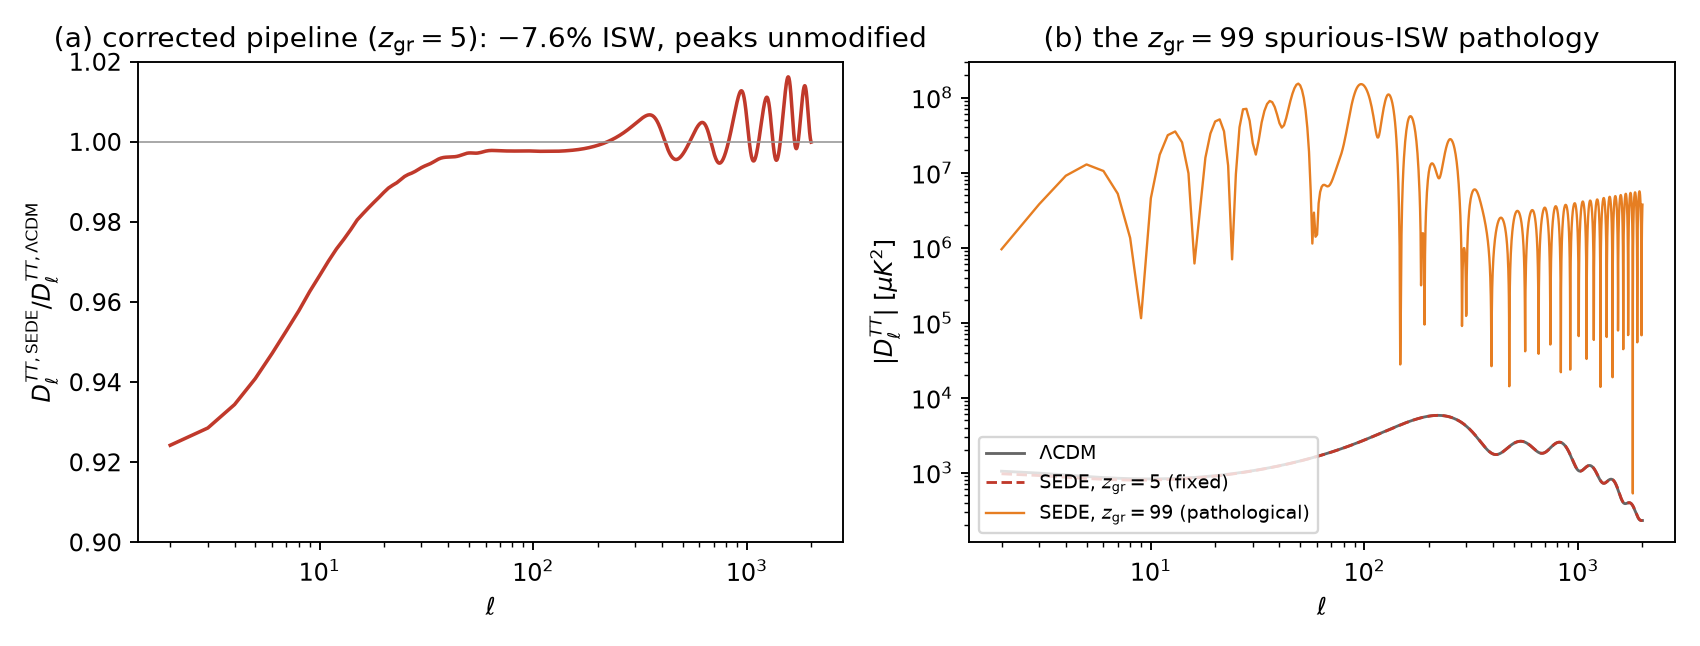
\includegraphics[keepaspectratio]{figures/solver_pathology_isw.png}}
\caption{(a) The corrected \(\mathrm{SEDE}/\Lambda \mathrm{CDM}\)
temperature-spectrum ratio \((z_{\mathrm{gr}} = 5)\): the \(-7.6\)\% ISW
deficit at ℓ = 2, recovering to within 0.5\% of unity by ℓ ≈ 50, with
the acoustic peaks unmodified. (b) The same model computed at
\(z_{\mathrm{gr}} = 99\): the spurious scalar oscillation injects a fake
ISW that corrupts the spectrum by up to three orders of
magnitude.}\label{fig:1}
\end{figure}

\section{Background-level comparison: BAO + SN (+ BBN)}\label{sec-4}

Direct multi-start minimization (Nelder--Mead \(\to\) Powell; four
starts agreeing to better than \(10^{-3}\)) over \{\(H_{0}\),
\(\omega _{\mathrm{b}}\), \(\omega _{\mathrm{cdm}}\)\}:

\begin{longtable}[]{@{}
  >{\raggedright\arraybackslash}p{(\linewidth - 12\tabcolsep) * \real{0.1429}}
  >{\raggedright\arraybackslash}p{(\linewidth - 12\tabcolsep) * \real{0.1429}}
  >{\raggedright\arraybackslash}p{(\linewidth - 12\tabcolsep) * \real{0.1429}}
  >{\raggedright\arraybackslash}p{(\linewidth - 12\tabcolsep) * \real{0.1429}}
  >{\raggedright\arraybackslash}p{(\linewidth - 12\tabcolsep) * \real{0.1429}}
  >{\raggedright\arraybackslash}p{(\linewidth - 12\tabcolsep) * \real{0.1429}}
  >{\raggedright\arraybackslash}p{(\linewidth - 12\tabcolsep) * \real{0.1429}}@{}}
\toprule\noalign{}
\begin{minipage}[b]{\linewidth}\raggedright
model
\end{minipage} & \begin{minipage}[b]{\linewidth}\raggedright
\(\chi ^{2}\)
\end{minipage} & \begin{minipage}[b]{\linewidth}\raggedright
\(\chi ^{2}_\mathrm{BAO}\)
\end{minipage} & \begin{minipage}[b]{\linewidth}\raggedright
\(\chi ^{2}_\mathrm{SN}\)
\end{minipage} & \begin{minipage}[b]{\linewidth}\raggedright
\(H_{0}\)
\end{minipage} & \begin{minipage}[b]{\linewidth}\raggedright
\(\omega _{\mathrm{cdm}}\)
\end{minipage} & \begin{minipage}[b]{\linewidth}\raggedright
\(\Omega _{\mathrm{m}}\)
\end{minipage} \\
\midrule\noalign{}
\endhead
\bottomrule\noalign{}
\endlastfoot
\(\Lambda \mathrm{CDM}\) & 1416.18 & 10.89 & 1405.29 & 68.76 & 0.1215 &
0.305 \\
SEDE & 1415.75 & 10.75 & 1405.00 & 69.13 & 0.1248 & 0.306 \\
\end{longtable}

\textbf{\(\Delta \chi ^{2} = -0.43\)} (this is the BAO+SN+BBN background
statistic; the companion's \emph{full-CMB profiled} fit lands on the
same number coincidentally --- a different test): geometrically
indistinguishable, with SEDE preferring \(H_{0}\) higher by 0.4. This is
the expected null --- SEDE's discriminating physics is in the
perturbations, not the distances.

\section{Full-likelihood comparison}\label{sec-5}

\textbf{Best fit.} Multi-start scipy minimization over the five
non-prior-pinned parameters (the cobaya Nelder-Mead wrapper stalls at
its reference simplex in this setup; the direct minimization is robust,
both starts per model agreeing to \textless{} 0.1):

\begin{longtable}[]{@{}
  >{\raggedright\arraybackslash}p{(\linewidth - 16\tabcolsep) * \real{0.1111}}
  >{\raggedright\arraybackslash}p{(\linewidth - 16\tabcolsep) * \real{0.1111}}
  >{\raggedright\arraybackslash}p{(\linewidth - 16\tabcolsep) * \real{0.1111}}
  >{\raggedright\arraybackslash}p{(\linewidth - 16\tabcolsep) * \real{0.1111}}
  >{\raggedright\arraybackslash}p{(\linewidth - 16\tabcolsep) * \real{0.1111}}
  >{\raggedright\arraybackslash}p{(\linewidth - 16\tabcolsep) * \real{0.1111}}
  >{\raggedright\arraybackslash}p{(\linewidth - 16\tabcolsep) * \real{0.1111}}
  >{\raggedright\arraybackslash}p{(\linewidth - 16\tabcolsep) * \real{0.1111}}
  >{\raggedright\arraybackslash}p{(\linewidth - 16\tabcolsep) * \real{0.1111}}@{}}
\toprule\noalign{}
\begin{minipage}[b]{\linewidth}\raggedright
model
\end{minipage} & \begin{minipage}[b]{\linewidth}\raggedright
\(\chi ^{2}\) total
\end{minipage} & \begin{minipage}[b]{\linewidth}\raggedright
BAO
\end{minipage} & \begin{minipage}[b]{\linewidth}\raggedright
SN
\end{minipage} & \begin{minipage}[b]{\linewidth}\raggedright
lowl TT
\end{minipage} & \begin{minipage}[b]{\linewidth}\raggedright
TTTEEE-lite
\end{minipage} & \begin{minipage}[b]{\linewidth}\raggedright
\(H_{0}\)
\end{minipage} & \begin{minipage}[b]{\linewidth}\raggedright
\(\omega _{\mathrm{cdm}}\)
\end{minipage} & \begin{minipage}[b]{\linewidth}\raggedright
\(n_{\mathrm{s}}\)
\end{minipage} \\
\midrule\noalign{}
\endhead
\bottomrule\noalign{}
\endlastfoot
\(\Lambda \mathrm{CDM}\) & 2023.61 & 11.53 & 1406.00 & 22.86 & 583.22 &
68.53 & 0.1185 & 0.9682 \\
SEDE & 2020.18 & 11.19 & 1406.70 & 22.38 & \textbf{579.91} & 68.86 &
0.1193 & 0.9664 \\
\end{longtable}

\textbf{\(\Delta \chi ^{2}(\mathrm{SEDE}-\Lambda \mathrm{CDM}) = -3.4\)},
dominated by the high-ℓ TTTEEE term \((-3.3)\). (This minimization
predates the BBN prior of Section~\ref{sec-2} and fixes \(\tau\) and
\(A_{\mathrm{planck}}\): \(\omega _{\mathrm{b}}\) sits at its box edge,
0.0225, for \emph{both} models --- identical treatment, so the
\emph{model difference} is a fair comparison, but this best fit lives on
a different likelihood than the with-BBN, \(\tau\)-sampled MCMC below,
so the two should be read as separate checks of the same direction, not
as the same statistic evaluated three ways.) We emphasize an instructive
false trail: evaluated at \(\Lambda \mathrm{CDM}'s\) own best fit,
SEDE's high-ℓ \(\chi ^{2}\) is \textasciitilde200 \emph{worse} --- the
imprint of \(\mu _\infty  = 1.05\) over-lensing the damping tail. That
apparent tension is an artifact of the comparison point: the joint refit
absorbs it entirely through small shifts \((n_{\mathrm{s}} -0.002\),
\(\omega _{\mathrm{cdm}} +0.0008\), \(H_{0} +0.33\)), leaving a net
\emph{gain}. We flag the fragility honestly: \(a -3.4\) that is the
residual of a \textasciitilde200-unit cancellation along the
\(\omega _{\mathrm{cdm}}/H_{0}/n_{\mathrm{s}}\) degeneracy is sensitive
to the joint minimum for \emph{both} models, and our Nelder--Mead
tolerance (both starts agreeing to \textless{} 0.1) is not far below the
signal; the marginalized \(\Delta \mathrm{DIC}\) (below) is the robust
statement, the best-fit \(-3.4\) the fragile one. Physically, SEDE's
extra lensing points the \emph{same way as} Planck's mild
\(A_{\mathrm{lens}} > 1\) tendency
\citep{Planck:2018vyg, Calabrese:2008rt} --- which is precisely the
concern: \(A_{\mathrm{lens}} > 1\) is at least partly a lite-likelihood
systematic --- the peak-smoothing excess is not seen in the direct
lensing reconstruction
\citep{Motloch:2018pjy, Motloch:2019gux, Addison:2023fqc} and it relaxes
toward unity in PR4/CamSpec and with ACT DR6
\citep{AtacamaCosmologyTelescope:2025blo} --- so a preference
concentrated in exactly that channel could be \emph{absorbing} that
systematic rather than detecting lensing physics. Distinguishing the two
requires the Planck lensing \((\phi \phi )\) likelihood, which the
lensing-shaped gain specifically predicts (§\ref{sec-7}) --- until it is
run, the physical interpretation of the \(-3.5\) is provisional.
\(A_{\mathrm{s}}\) alone cannot mimic the effect (lowering
\(A_{\mathrm{s}}\) degrades the primary peaks).

\textbf{Marginalized (production MCMC).} Converged chains for both
models \((R-1\) means: 0.014 / 0.015; bounds \textless{} 0.11; 13.0k /
19.6k accepted samples; learned proposal seeded from the Planck
\texttt{base\_plikHM\_TTTEEE\_lowl\_post\_BAO} covariance; spectral
guard active throughout, zero rejections):

\begin{longtable}[]{@{}lll@{}}
\toprule\noalign{}
& \(\Lambda \mathrm{CDM}\) & SEDE \\
\midrule\noalign{}
\endhead
\bottomrule\noalign{}
\endlastfoot
\(H_{0}\) & 68.54 ± 0.29 & 68.89 ± 0.30 \\
\(\omega _{\mathrm{cdm}}\) & 0.11847 ± 0.00063 & 0.11922 ± 0.00066 \\
\(n_{\mathrm{s}}\) & 0.9685 ± 0.0032 & 0.9665 ± 0.0033 \\
\(10^{9}A_{\mathrm{s}}\) (from log A) & 2.113 ± 0.031 & 2.112 ± 0.032 \\
\(\langle\chi^2\rangle\) & 2028.1 & 2025.1 \\
\(p_{\mathrm{D}}\) & 6.8 & 6.3 \\
\textbf{DIC} & 2034.9 & \textbf{2031.4} \\
\end{longtable}

\begin{equation}\Delta\mathrm{DIC}(\mathrm{SEDE}-\Lambda\mathrm{CDM}) = -3.5\end{equation}

With identical priors and the same parameter count, this is a
marginalized, real-likelihood statement that SEDE fits the joint dataset
mildly better --- ``positive but not strong'' evidence in the DIC 2--5
band \citep{Spiegelhalter:2002bk} (we attach no \(\sigma\)-level: the
models are non-nested and \(\Delta \mathrm{DIC}\) is not
\(\chi ^{2}\)-distributed). The \(p_{\mathrm{D}}\) difference (6.8 vs
6.3) is within the Monte-Carlo scatter of \(p_{\mathrm{D}}\) at these
chain lengths and the posterior widths are nearly identical, so we read
this \emph{pre-lensing} number as
\(\Delta \mathrm{DIC} \approx  \Delta\)\(\langle\chi^2\rangle\) ≈ −3.0
rather than resting on a half-unit of effective-complexity difference.
The best-fit \(-3.4\) and the marginalized \(-3.5\) point the same way
but are computed on different likelihoods (above); we treat the
marginalized \(\Delta \mathrm{DIC}\) as the pre-lensing headline ---
folding in the direct \(\phi \phi\) datum below reduces it to \(-2.3\),
which is the number we ultimately quote. (The companion's compressed
CAMB-in-the-loop pipeline gives a related full-CMB
\(\Delta \chi ^{2} = -3.17\) on its wider
\(\mathrm{DESI}+\mathrm{SN}+\mathrm{CC}+f\sigma 8\) data vector; the
\(-3.4\) here is the independent mochi-class best-fit on the
DESI+SN+Planck vector.) SEDE's posterior pulls \(H_{0}\) upward by +0.35
\((0.8\sigma\) of the combined width) --- the right direction for the
\(H_{0}\) tension, at an inconsequential magnitude. The joint posterior
shifts are shown in Fig. 2.

\begin{figure}
\centering
\pandocbounded{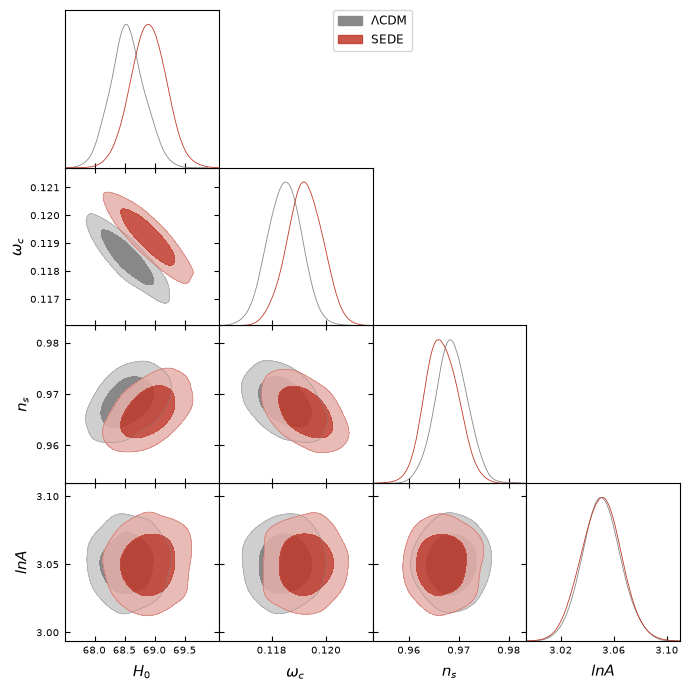
\includegraphics[keepaspectratio]{figures/sede_lcdm_mcmc_triangle.png}}
\caption{Marginalized posteriors (68\% and 95\%) for \(H_{0}\),
\(\omega _{\mathrm{cdm}}\), \(n_{\mathrm{s}}\) and log
\(A_{\mathrm{s}}\): \(\Lambda \mathrm{CDM}\) (grey) vs SEDE (red). The
coherent small shifts \((H_{0}\) up, \(n_{\mathrm{s}}\) down,
\(\omega _{\mathrm{cdm}}\) up) are how SEDE accommodates its extra
lensing.}\label{fig:2}
\end{figure}

\textbf{The Planck-lensing \((\phi \phi )\) cross-check.} The preference
above lives entirely in the high-ℓ TTTEEE smoothing, in the direction of
Planck's \(A_{\mathrm{lens}}\) tendency --- which is partly a
lite-likelihood systematic (above, and §\ref{sec-7}). The direct Planck
2018 lensing \((\phi \phi )\) likelihood \citep{Planck:2018lbu}, whose
reconstructed amplitude sits at \(\approx 1.0\) rather than the
TT-derived \(\approx 1.2\), decides whether SEDE's extra smoothing is
physical lensing or an absorbed systematic --- the same
peak-smoothing-vs-reconstruction consistency test used
model-independently by Planck and by Motloch \& Hu
\citep{Motloch:2018pjy, Motloch:2019gux}, here applied to SEDE --- so we
ran it. We refit \emph{both} models over \{\(H_{0}\),
\(\omega _{\mathrm{b}}\), \(\omega _{\mathrm{cdm}}\),
\(A_{\mathrm{s}}\), \(n_{\mathrm{s}}\)\} to the full DESI DR2 BAO +
Pantheon+ + BBN + lowl TT + TTTEEE data --- once without and once with
\texttt{planck\_2018\_lensing.native} (CMB-marginalized). Without
\(\phi \phi\) the joint preference is \(\Delta \chi ^{2} = -3.5\)
(reproducing the best fit and the DIC); \textbf{with \(\phi \phi\) it is
\(\Delta \chi ^{2} = -2.3\)}. SEDE fits \(\phi \phi\) \emph{worse} than
\(\Lambda \mathrm{CDM}\) by +1.2 \((\chi ^{2}_\phi \phi  = 10.0\) vs
8.8), because \(\mu _\infty  = 1.05\) boosts \(C_\ell ^{\phi \phi }\)
above the measured amplitude; the direct lensing datum thus
\textbf{erodes the preference from \(-3.5\) to \(-2.3\)} \((\)≈⅓; 66\%
survives), so about a third of the high-ℓ TTTEEE gain is
\emph{consistent with} the absorbed \(A_{\mathrm{lens}}\) systematic
rather than physical lensing (the test cannot separate an absorbed
systematic from \(\mu _\infty\) over-predicting real lensing). Because
BAO + SN + BBN pin the background density
\((\omega _{\mathrm{cdm}} \approx  0.119\) in both fits), this anchored
joint refit is the honest number: a CMB-primary-only refit that frees
\(\omega _{\mathrm{cdm}}\) gives a smaller penalty (+0.3) \emph{only} by
letting \(\Lambda \mathrm{CDM}'s\) \(\omega _{\mathrm{cdm}}\) drift to
an unphysical 0.120, and an \(A_{\mathrm{s}}\)-profiled evaluation at
the primary optimum gives −1.9 as a conservative (off-minimum) upper
bound --- the anchored joint refit at \(-2.3\) supersedes both. The
\(\phi \phi\) likelihood is CMB-marginalized, so it shares some Planck
TT information and is not a fully independent datum, and
\(\chi ^{2}_\phi \phi (\Lambda \mathrm{CDM}) \approx  8.8\) is
consistent with (not a proof of) a well-calibrated ∼9-bandpower
likelihood. This is the direct evidence behind the ``consistent with
\(\Lambda \mathrm{CDM}\), mild pull'' reading (repro
\texttt{phiphi\_joint\_refit.py}; earlier estimates and caveats in
\texttt{results/phiphi\_test\_result.md}).

\section{Predictions}\label{sec-6}

The comparison above is a consistency statement; the model's falsifiable
content is forward-looking. We separate it by robustness: the growth
signal (1) is fixed by the sub-horizon coupling \(\mu _\infty\), set
above the tachyonic window and independent of the solver's GR-transition
regularization --- this is the \textbf{primary pre-registered test}; the
ISW signal (2) is computed \emph{below} the window and is
correspondingly more model-dependent, a \textbf{corroborating} rather
than a primary falsifier.

\begin{enumerate}
\def\labelenumi{\arabic{enumi}.}
\tightlist
\item
  \textbf{Growth (primary falsifier).}
  \(P_\mathrm{SEDE}/P_\Lambda \mathrm{CDM} = +2.6\)\%, flat across k =
  0.01--1 h/Mpc; \(\sigma 8\) ratio +1.3\%; and a \textbf{+2--3\%
  scale-independent \(f\sigma 8\) enhancement through the RSD range}
  (Fig. 3; from the sub-horizon coupling \(\mu _\infty  = 1.05\), fixed
  by \(\alpha _{\mathrm{B0}}\) and independent of the tachyonic-window
  regularization; k-table: +2.9/+2.3/+2.0/+1.7\% at z = 0/0.3/0.5/1 for
  k = 0.1 h/Mpc). Current \(f\sigma 8\) errors are 5--8\%; DESI DR3 and
  Euclid reach the 2--3\% level. \textbf{The sign is opposite to what
  would ease the \(S_{8}\) tension}, and opposite to the mild
  \emph{suppression} of growth \((\gamma  > 0.55)\) current data prefer
  \citep{Nguyen:2023fip} --- this prediction is a genuine risk, not an
  accommodation. An \(f\sigma 8\) measured \emph{not} enhanced at this
  level falsifies the \(\mu (k)\) sector (pre-registered as P5 --- the
  growth+ISW signature --- of the program's frozen P1--P20 falsifier
  matrix; not to be confused with the cosmology paper's \emph{internal}
  prediction numbering, whose P3--P5 are the withdrawn SOC layer).
\item
  \textbf{ISW (corroborating).} \(C_\ell ^\mathrm{TT}\) ratio 0.924 at ℓ
  = 2, 0.987 at ℓ = 20, within 0.5\% of unity by ℓ ≈ 50: \(a -7.6\)\%
  low-ℓ deficit, cosmic-variance-limited but contributing to low-ℓ TT
  likelihoods and to ISW--LSS cross-correlations. Because it is computed
  below the tachyonic window (§\ref{sec-3}), this prediction is more
  model-dependent than the growth signal and should be read as
  corroborating it, not as an independent primary falsifier. This is
  also where FPAB-SEDE separates cleanly from the cubic-Galileon models
  excluded at ∼7--\(8\sigma\) by the ISW--galaxy cross-correlation
  \citep{Renk:2017rzu}: that exclusion targets \emph{self-accelerating}
  Galileons, whose kinetic term drives the acceleration and flips the
  sign of the \(\mathrm{ISW}\times galaxy\) cross-power
  (anti-correlation). FPAB-SEDE is \textbf{not} self-accelerating ---
  the acceleration is carried by the background
  \(\rho _\mathrm{DE} \propto  H\) \(f_{\mathrm{sat}}\), and the
  braiding is a weak \((b \approx  0.2\), \(\mu _\infty  = 1.05\))
  sub-horizon correction --- so its \(\mathrm{ISW}\times galaxy\)
  cross-power keeps the \(\Lambda \mathrm{CDM}\) sign and is mildly
  \emph{enhanced} (+13\% at ℓ = 2, with the \(-7.6\)\% temperature-auto
  deficit above being the standard auto-vs-cross sign structure of a
  stronger late-ISW source; cosmology paper §\ref{sec-7}). SEDE
  therefore evades the Renk et al.~exclusion by construction rather than
  by tuning.
\item
  \textbf{DE clustering.}
  \(\delta _\mathrm{DE}/\delta _{\mathrm{m}} \lesssim  7\times 10^{-5}\)
  at k = 0.1 h/Mpc (horizon-confined): any detected gate--matter
  cross-correlation at RSD scales kills the realization outright.
\end{enumerate}

\begin{figure}
\centering
\pandocbounded{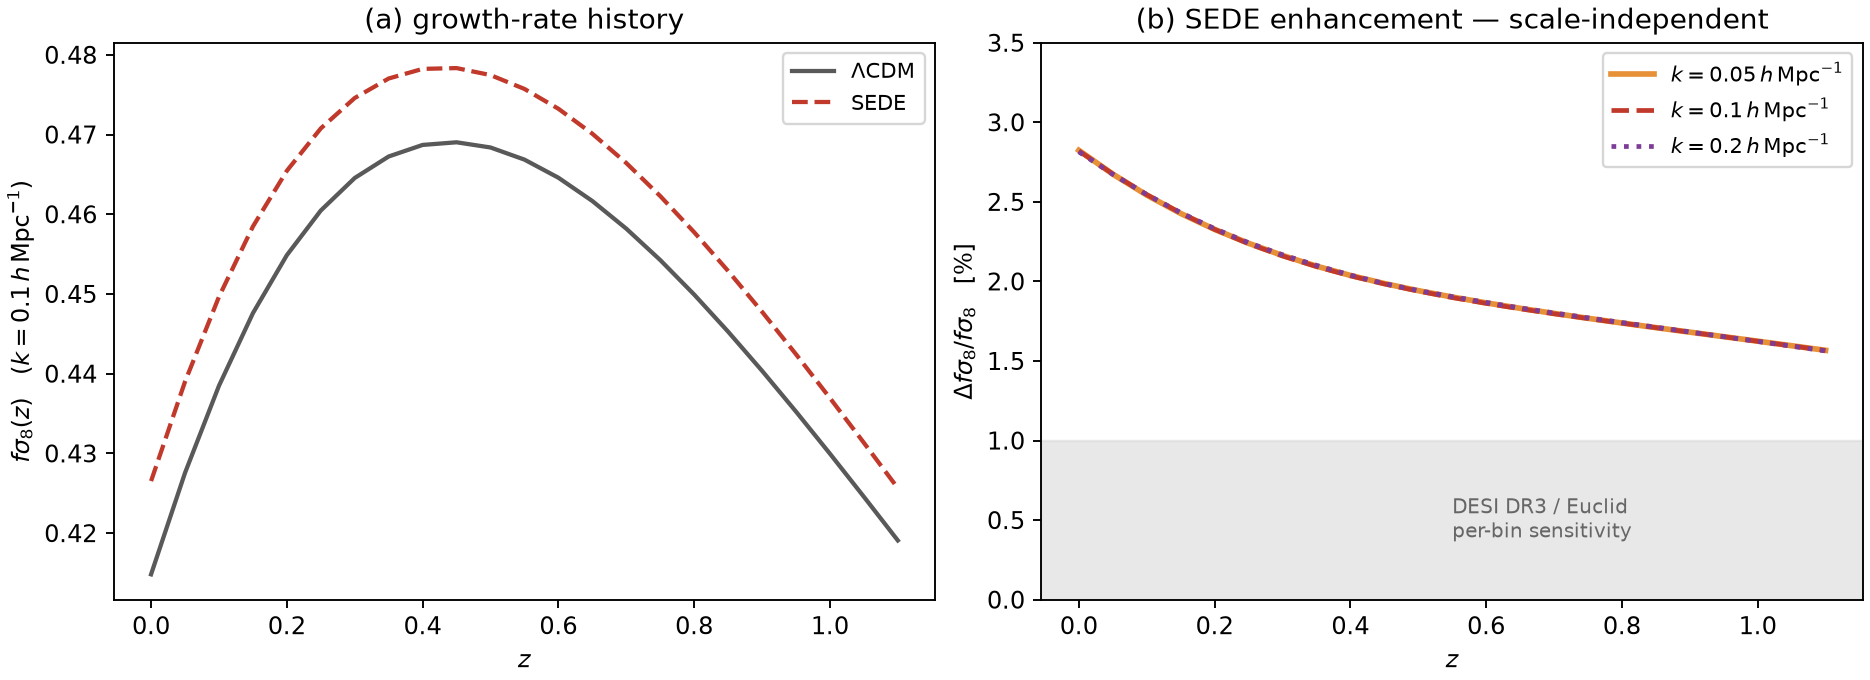
\includegraphics[keepaspectratio]{figures/fsigma8_prediction.png}}
\caption{The growth prediction. (a) \(f\sigma 8(z)\) at k = 0.1 h/Mpc
for \(\Lambda \mathrm{CDM}\) and SEDE at the shared best-fit cosmology.
(b) The fractional SEDE enhancement at k = 0.05, 0.1 and 0.2 h/Mpc ---
the three curves lie on top of one another, which is the point: the
enhancement is scale-independent through the RSD range, entering the
DESI DR3/Euclid sensitivity band. Underlying data:
\texttt{src/fsigma8\_prediction.json}, regenerated by
\texttt{src/sims/sede\_fsigma8\_isw\_finitek.py}.}\label{fig:3}
\end{figure}

\section{Limitations}\label{sec-7}

\begin{itemize}
\tightlist
\item
  \(\Delta \mathrm{DIC} = -3.5\) (robust part
  \(\Delta\)\(\langle\chi^2\rangle\) ≈ −3.0) is positive, not decisive;
  the data are statistically consistent with \(\Lambda \mathrm{CDM}\)
  and we make no detection claim.
\item
  \textbf{We ran the decisive test --- the Planck lensing
  \((\phi \phi )\) likelihood --- and it pulls the preference down.} The
  entire preference sits in the high-ℓ TTTEEE term, where Planck's
  \(A_{\mathrm{lens}} > 1\) tendency lives. Adding the direct
  \(\phi \phi\) likelihood (\texttt{planck\_2018\_lensing.native},
  reconstructed amplitude \(\approx  1.0\)) in a full
  BAO/SN/BBN-anchored joint refit erodes the preference from \(-3.5\) to
  \textbf{−2.3} (§\ref{sec-5}): about a third of the TTTEEE gain is
  consistent with the absorbed \(A_{\mathrm{lens}}\) systematic rather
  than physical lensing. Repeating against a PR4/CamSpec or ACT high-ℓ
  likelihood (where \(A_{\mathrm{lens}} \approx  1\)), and the full
  multi-nuisance plik (vs the lite used here) with \(\phi \phi\) in the
  marginalized chains, are the remaining checks --- expected to point
  the same way. \(The -3.5\) is thus a pre-\(\phi \phi\) upper bound;
  the direct lensing datum reads the preference down to −2.3.
\item
  No w0waCDM baseline is run here: SEDE's selling point (same physics,
  zero extra parameters) is best shown against the 2-extra-parameter
  parametric alternative; the \((w_{0}\),wₐ) placement is in the
  companion (∼\(2.7\sigma\) from the DESI point, ∼\(0.5\sigma\) from
  \(\Lambda \mathrm{CDM}\)), and a direct w0waCDM
  \(\Delta \mathrm{DIC}\) is deferred.
\item
  One Boltzmann implementation (one fork) computed everything; an
  independent EFT code (e.g.~EFTCAMB \citep{Hu:2013twa}) reproducing the
  \(\mu _\infty /\mathrm{ISW}\) numbers would remove a
  single-implementation systematic.
\item
  The solver operates \emph{below} the reconstruction's tachyonic window
  rather than through it. The window is a genuine long-wavelength
  (Jeans-type) instability --- though \emph{not} a ghost or gradient one
  \((D_{\mathrm{kin}} > 0\) and \(c_{\mathrm{s}}^{2} > 0\) throughout,
  §\ref{sec-3}), which is why regularizing it by seeding below the
  window is legitimate rather than a suppression of healthy physics;
  whether the window itself is a real feature of the reconstructed EFT
  or an artifact of the Chebyshev inversion deserves a dedicated study.
  The sub-horizon growth signal \((\mu _\infty\), \(f\sigma 8\)) is set
  \emph{above} the window and is insensitive to this question; the ISW
  and the lensing-shaped −3.3, computed \emph{below} it, are conditional
  on it --- one further reason we take the \(f\sigma 8\) prediction, not
  the ISW or the \(-3.5\), as the primary falsifiable claim.
\item
  The background and stability inputs are frozen at b = 0.20; the
  braiding fraction is a free parameter of the wider program (forecast
  measurable at \textasciitilde{}\(5\sigma\) by DR3+Euclid), not varied
  here.
\end{itemize}

\section{Conclusions}\label{sec-8}

At equal parameter count against the real likelihoods, structure-gated
dark energy is \textbf{statistically consistent with
\(\Lambda \mathrm{CDM}\)}, with a mild same-direction pull (marginalized
\(\Delta \mathrm{DIC} = -3.5\), of which the robust part is
\(\Delta\)\(\langle\chi^2\rangle\) ≈ −3.0 --- ``positive but not
strong'' evidence). The pull sits entirely in the lensing-scale
smoothing of the Planck damping tail, in the direction of Planck's
\(A_{\mathrm{lens}}\) tendency; because that tendency is itself partly a
lite-likelihood systematic, we ran the decisive test --- the direct
Planck lensing \((\phi \phi )\) likelihood (§\ref{sec-5}) --- in a full
BAO/SN/BBN-anchored joint refit it pulls the preference down from
\(-3.5\) to \textbf{−2.3}: about a third of the gain is consistent with
the absorbed \(A_{\mathrm{lens}}\) systematic rather than physical
lensing. We make no detection claim. What makes the model falsifiable on
a short horizon is not this pull but its forward predictions, led by the
one independent of the solver regime: a +2--3\% sub-horizon
\(f\sigma 8\) enhancement that DESI DR3/Euclid can confirm or kill,
corroborated by an ISW deficit, and a strict null in gate--matter
correlations at sub-horizon scales. Within these caveats the
compressed-CMB comparison of the companion paper is reproduced ---
SH0ES-free --- by this full-likelihood analysis: both give a mild,
same-sign, non-decisive pull, the full-likelihood
\(\Delta \mathrm{DIC} \approx  -3.0\) sitting at the conservative end of
the companion's \(\Delta \mathrm{DIC} \approx  -3.5\) to −4.7 range
(whose upper end is carried by the contested SH0ES prior ---
\textasciitilde40\% of the companion's evidence --- and the
compression-vs-full dilution the companion itself reports, −4.68 \(\to\)
−3.17). Having now folded in the direct Planck lensing datum, we regard
\(-2.3\) as the honest post-\(\phi \phi\) preference --- mild,
same-sign, and firmly non-decisive.

\section*{Reproducibility}\label{reproducibility}
\addcontentsline{toc}{section}{Reproducibility}

The configurations, minimizers, the spectral guard, the diagnostic
scripts and the chains' SHA-256 checksums are in the
\href{https://github.com/spsingularity/sede-observational-tests}{\texttt{sede-observational-tests}}
repository; the production chain files, the minima, and the
chain\(\to\)(\(\langle\chi^2\rangle\), \(p_{\mathrm{D}}\), DIC)
reduction script are to be committed with the release, so that the
headline \(\Delta \mathrm{DIC}\) is auditable and not only rerunnable.
The Boltzmann engine is the pinned mochi-class fork (\texttt{74d4b05}
solver guard; \texttt{b365166} frozen FPAB inputs; build:
\texttt{rm\ python/classy.cpp\ \&\&\ pip\ install\ .\ -\/-no-build-isolation}).
The fork location is set via \texttt{MOCHI\_DIR}, the frozen SEDE inputs
are vendored in \texttt{src/mcmc/inputs/}, and likelihood data install
via \texttt{cobaya-install} from the included
\texttt{likes\_install.yaml} (full setup in \texttt{src/README.md}). The
growth/ISW predictions \((\sigma 8\), \(f\sigma 8\), the
\(C_\ell ^\mathrm{TT}(2)=0.924\) ISW ratio) regenerate directly from
\texttt{src/sims/sede\_fsigma8\_isw\_finitek.py}; the production chains
were run with the exact \texttt{lcdm\_mc.yaml} / \texttt{sede\_mc.yaml}
released here (Rminus1 stop 0.02; the loose
\(Rminus1_{\mathrm{cl},\mathrm{stop}}\) 0.2 on the tails should be
tightened for the released run). The Planck-lensing \((\phi \phi )\)
test of §\ref{sec-5}: the definitive BAO/SN/BBN-anchored joint refit is
\texttt{src/mcmc/phiphi\_joint\_refit.py} (needs the full DESI DR2 BAO +
Pantheon+ + Planck primary + lensing data via \texttt{cobaya-install}),
giving \(\Delta \chi ^{2} = -3.5\) → −2.3 with \(\phi \phi\); the
earlier \(A_{\mathrm{s}}\)-profiled and CMB-only estimates
(\texttt{phiphi\_As.py}, \texttt{phiphi\_fullrefit.py}) and all caveats
are in \texttt{src/results/phiphi\_test\_result.md}.

\section*{Acknowledgements}\label{acknowledgements}
\addcontentsline{toc}{section}{Acknowledgements}

AI assistance: the analysis and drafting of this paper were carried out
with the assistance of Claude (Anthropic). All numerical claims trace to
the released, rerunnable configurations and scripts.
\bibliographystyle{JHEP}
\bibliography{refs}
\end{document}
